\chapter{Introduction}

Federated Learning ist ein Trainingsverfahren im Machine Learning bei dem Modelle lokal an dem Ort trainiert werden, an dem die Daten für das Training generiert werden. So kann einerseits vermieden werden sensible Daten an einen zentralen Server zu schicken und andererseits können Modelle weiter auf lokalen Daten optimiert werden, wie beispielsweise bei der Wortvorhersage für Smartphone-Tastaturen \parencite{mcmahan:2018}. 

Trotz der dezentralen Struktur bleiben mit Federated Learning (FL) Privacy Risiken bestehen. Beispielsweise kann Federated Learning Membership Inference Attacks nicht vermeiden. Differential Privacy (DP) dagegen kann diese sehr wohl verhindern \parencite{shokri:2017}. 

Allerdings führt die Anwendung von DP zu einem Utility-Privacy Tradeoff. Zwar haben \textcite{mcmahan:2018} gezeigt, dass die Genauigkeit auch unter DP-Garantien beibehalten werden kann, allerdings zum Preis von bedeutend mehr Trainingsaufwand. Individuelle Privacy Budgets können dazu beitragen, den Verlust an \textit{Utility} zu minimieren. Bei klassischen DP-Trainingsalgorithmen wird an alle Daten die gleiche Privacy-Anforderung angelegt. Da verschiedene Personen in der Realität verschiedene Privacy-Anforderungen an ihre Daten haben, sind die strengsten Anforderungen unnötig strikt für einen großen Teil der Daten. Dadurch kann die Utility, also die Fähigkeit aus den Daten zu lernen, deutlich verschlechtert werden. Um diese Heterogenität in den Anforderungen besser abzubilden wird an Algorithmen geforscht, die diese heterogenen Privacy-Budgets optimal ausnutzen.

Das Ziel dieser Arbeit ist die Entwicklung und Evaluation eines Trainingsalgorithmus in einem Federated Learning Szenario unter Beachtung von individuellen Privacy Budgets. Die verschiedenen Clients haben dabei individuelle Privacy Budgets für ihre Trainingsdaten. Ziel ist dabei nicht der Schutz der Clients vor dem aggregierenden Server, sondern am Ende des Trainingsprozesses ein Modell zu erhalten, das die individuellen Privacy Budgets einhält.

\section{Differential Privacy}

Differential Privacy ist ein Konzept zur Einhaltung von Privacy bei der Verarbeitung von sensiblen Daten, das von \textcite{dwork:2006} eingeführt wurde. Im Grundsatz wird dabei Rauschen auf Anfrageergebnisse addiert, um zu garantieren, dass das Anfrageergebnis bei einem \textit{benachbarten Datensatz} mit einer ähnlichen Wahrscheinlichkeit auftreten würde. So wird garantiert, dass der Einfluss eines einzelnen Datenpunktes auf das Anfrageergebnis begrenzt ist. Die Ähnlichkeit der Wahrscheinlichkeiten wird dabei durch das \textit{Privacy Budget} $\epsilon$ festgelegt. Eine weniger strenge, aber in der Praxis viel genutzte Definition führt darüber hinaus ein $\delta \in [0,1]$ ein, das eine Wahrscheinlichkeit dafür liefert, dass keine Privacy Garantien eingehalten werden. In \textcite{abadi:2016} wird Differential Privacy folgendermaßen definiert:

\begin{definition}
  \emph{\textbf{$(\epsilon, \delta)$-Differential Privacy}} A \textit{randomized mechanism} $\mathcal{M}: \mathcal{D} \rightarrow \mathcal{R}$ with domain $\mathcal{D}$ and range $\mathcal{R}$ satisfies $(\epsilon, \delta)$-differential privacy if for any two adjacent inputs $d$, $d' \in \mathcal{D}$ and for any subset of outputs $S \subseteq \mathcal{R}$ it holds that $$\Pr[\mathcal{M}(d) \in S] \leq e^{\epsilon} \Pr[\mathcal{M}(d') \in S] + \delta$$
\end{definition}

Auf Basis dieser Definition gibt es weitere Theoreme, die die Entwicklung von komplexeren DP-Algorithmen ermöglichen. Das erste ist das \textit{Post Processing}-Theorem. Es besagt, dass die Weiterverarbeitung von Daten aus einem DP-Mechanismus den Privacy-Verlust nicht weiter erhöhen kann. Diese Eigenschaft ist wichtig, um beispielsweise mit Privacy Garantien trainierte Modelle nach dem Training bedenkenlos nutzen zu können. Darüber hinaus gibt es Kompositionstheoreme, die Abschätzungen dafür liefern, dass Daten mehrfach verarbeitet werden.

Das Rauschen wird durch verschiedene Mechanismen hinzugefügt. Dafür werden Zufallswerte aus Verteilungen gezogen, für die bewiesen ist, dass sie die Definition von Differential Privacy erfüllen. Für numerische Anfragen gibt es dafür der Laplace-Mechanismus, der die Zufallswerte aus der Laplace-Verteilung zieht und der Gausssche Mechanismus, der die Zufallswerte aus der Normalverteilung zieht. Für kategorische Anfragen ist beispielsweise der Exponential Mechanism geeignet. Weitere Details werden u.a. von \textcite{chang:2023} beschrieben.

Da die Stärke des hinzugefügten Rauschens proportional zu dem größtmöglichen Einfluss eines Datenpunktes auf das Anfrageergebnis sein sollte, ist es darüber hinaus häufig nötig den Wertebereich zu begrenzen \parencite[p.31]{chang:2023}. Bei Count-Anfragen ist dieser Einfluss natürlich auf $1$ begrenzt, wenn allerdings ein Durchschnittsgehalt angefragt wird, wird es nötig den Wertebereich der möglichen Gehälter festzulegen. Der größtmögliche Einfluss eines Datenpunkts wird hierbei \textit{Sensitivity} genannt.

\section{Differential Privacy in Machine Learning}

Auch Machine Learning Modelle können als Anfragen auf einen Datensatz angesehen werden. Bei ihnen kann ein DP-Mechanismus zu verschiedenen Zeitpunkten angewandt werden, wie in \autoref{fig:design_principles_dpml} zu sehen ist. Das hinzufügen von Rauschen in den jeweiligen Schritten hat verschiedene Vor- und Nachteile.

\begin{figure}[tb]
  \centering
  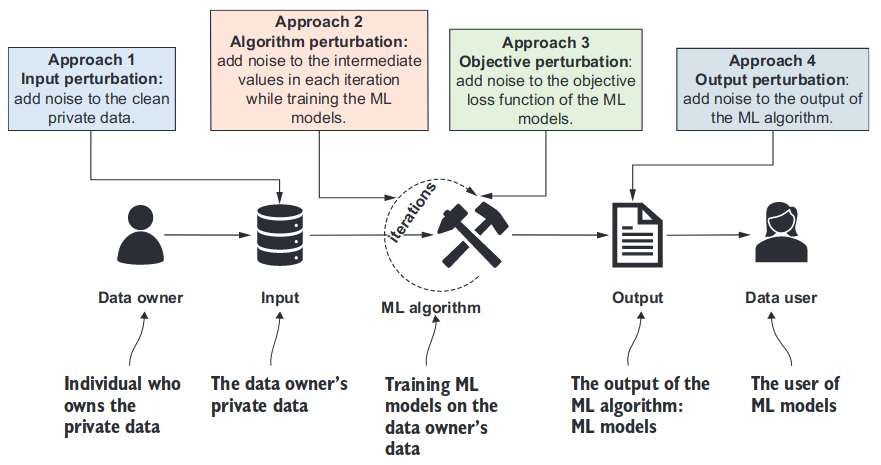
\includegraphics[width=0.7\textwidth]{Bilder/design_principles_dpml.png}
  \caption{Design principles of differentially private ML from \textcite{chang:2023}}
  \label{fig:design_principles_dpml}
\end{figure}

Bei der \textit{Input pertubation} wird den Trainingsdaten vor dem Training Rauschen hinzugefügt. Dies ist einfach zu implementieren und vielseitig einsetzbar, allerdings wird auch ein größeres Rauschen benötigt, da die Daten i.d.R. eine hohe \textit{Sensitivity} haben.

Bei der \textit{Algorithm pertubation} werden die Modelle mit unveränderten Daten trainiert. Bei iterativen Algorithmen können die Zwischenergebnisse in der einzelnen Schritte verändert werden. Bei \textcite{abadi:2016} werden beispielsweise den Gradienten Rauschen hinzugefügt.

Bei der \textit{Output pertubation} werden den vom Modell generierten Ausgaben hinzugefügt. Allerdings ist das Verfahren nicht anwendbar, wenn dass Modell veröffentlicht werden soll, da sich die Anzahl der Anfragen an das Modell nicht vorhersagen lässt und dadurch keine Privacy Garantien möglich sind.

Bei der \textit{Objective pertubation} wird der \textit{Objective function}, auf die das Modell optimiert wird, Rauschen hinzugefügt.

Der von \textcite{abadi:2016} vorgestellte Differentially Private-Stochastic Gradient Descent (DP-SGD) ist inzwischen ein viel genutzter Algorithmus für das Training von Neuronalen Netzen, auf dem viele weitere Arbeiten aufbauen. Grundlage ist der \textit{Stochastic Gradient Descent} (SGD), ein iterativer Optimierungsalgorithmus, der bei verschiedenen Machine Learning Verfahren genutzt wird. Im Vergleich zu dem SGD hat der DP-SGD einige zusätzliche Hyperparameter um die Privacy-Garantien zu erfüllen:

\begin{itemize}
  \item \textbf{Noise scale $\sigma$} Ein Faktor, mit dem das Rauschen des DP-Mechanismus gesteuert wird. 
  \item \textbf{Lot size $L$} Die Anzahl der Datenpunkte, die in ein Gradientenupdate einfließen.
  \item \textbf{Gradient norm bound $C$} Alle berechneten Gradienten werden so beschnitten, dass sie eine maximale $\ell_2$-Norm von $C$ haben. Das ist nötig, da im folgenden Rauschen mit dem Gausschen Mechanismus hinzugefügt wird und bei diesem die Sensitivität von Vektoren über die $\ell_2$-Norm definiert ist. 
\end{itemize}

Beim Training wirken sich diese Parameter darauf aus, wie schnell ein gewünschtes $(\epsilon, \delta)$-Privacy Budget ausgeschöpft ist. In ihren Ergebnissen verdeutlichen \textcite{abadi:2016}, dass sich die Wahl dieser Parameter (neben den Parametern aus dem normalen SGD) unter einem festgelegten Privacy Budget auf die Genauigkeit des Modells auswirkt.

Über den konkreten Algorithmus hinaus haben \textcite{abadi:2016} mit dem \textit{Moments Accountant} ein Verfahren zur Abschätzung des Verlustes an Privacy beim Training entwickelt, der asympotisch deutlich genauer ist, als klassische Abschätzungen über Kompositionstheoreme. Diesen Nutzen weisen sie in ihrer Arbeit durch empirische Experimente nach.

\textcite{mcmahan:2018} entwickeln in ihrem Paper auf Grundlage von \textcite{abadi:2016} einen Variante des \textit{Federated Averaging} (FedAvg) Algorithmus \parencite{mcmahan:2016}, die DP-Garantien für die Nutzer gewährleistet. Ihr Ziel ist das Training eines LSTM zur \textit{Next-Word Prediction} auf Mobilen Endgeräten. Sie übertragen die Definition von benachbarten Datensätzen auf das Federated Learning, indem die Nachbarschaft durch das hinzufügen oder entfernen aller Daten eines Nutzers definieren. In ihren Experimenten zeigen sie, dass die Genauigkeit des Modells auch unter DP-Garantien aufrechterhalten werden kann, allerdings zu höheren Berechnungskosten.

Die wichtigsten Änderungen gegenüber dem nicht-privaten FedAvg sind eine beschränkte Sensitivität bei den Clients (durch Clipping) und bei dem Server (durch Schätzer der Aggregation mit einem beschränkten Wertebereich). Darüber hinaus fügt der Server dem aggregierten Update auf Basis der Sensitivität Rauschen hinzu.

\section{Differential privacy with heterogeneous privacy budgets}

\textcite{boenisch:2023} zeigen auf, dass die Annahme eines Privacy-Budgets für alle Datenpunkte die Möglichkeiten eines Modells von einem Datensatz zu lernen beschränkt, da das strengste Privacy-Budget für alle angenommen werden muss. In der Realität haben aber unterschiedliche Nutzer, die die Daten generieren, unterschiedliche Anforderungen an ihre Privacy. Sie liefern für das Training mit heterogenen Privacy-Budgets zwei Ansätze: der erste (\textbf{SAMPLE}) schöpft das Privacy-Budget von weniger privaten Datenpunkten aus, indem diese während des Trainings mit einer höheren Wahrscheinlichkeit gezogen werden. Der zweite Ansatz (\textbf{SCALE}) steuert das genutzte Privacy-Budget indem die \textit{Noise Multiplier} und \textit{Clipping Norms} individualisiert werden.

\textcite{aldaghri:2023} präsentieren einen Algorithmus, um in Federated Learning Szenarien von heterogenen Privacy Anforderungen zu profitieren. Ähnlich wie der \textbf{SCALE} Algorithmus von \textcite{boenisch:2023} nutzt er individuelle Noise Scales für jede Gruppe mit dem gleichen Privacy Niveau. Darüber hinaus werden nur zwei Abstufungen von Privacy Niveaus evaluiert, nämlich Clients ohne Privacy Anforderungen und Clients mit Privacy Anforderungen. Zum verfolgen des \textit{privacy loss} nutzen sie einen Moments Accountant aus \textcite{abadi:2016} für jede Gruppe von Cleints mit den gleichen Privacy Anforderungen.

\section{Method}

In dieser Arbeit soll der Sampling Ansatz von \textcite{boenisch:2023} an ein Federated Learning Szenario angepasst werden. Er ersetzt das \textit{Poisson Sampling} von \textcite{abadi:2016} durch ein Sampling der Daten, das abhängig von dem jeweiligen \textit{Privacy Budget} ist. Wie bei \textcite{aldaghri:2023} und \textcite{mcmahan:2018} ist auch bei meiner Arbeit das Ziel, die (heterogenen) DP-Garantien im endgültigen Modell einzuhalten. Insbesondere ist es daher nicht das Ziel, die Clients während des Trainings gegenüber dem aggregierenden Server zu schützen.

Um die Einhaltung zu gewährleisten, werde ich wie \textcite{boenisch:2023} und \textcite{aldaghri:2023} für jede Gruppe mit dem gleichen Privacy Budget einen Moments Accountant nutzen. Darüber hinaus werde ich den \textit{FedAvg} Algorithmus nutzen, der auch bei \textcite{aldaghri:2023} die Grundlage ist.

Wichtige Fragen werden im Verlauf meiner Arbeit folgende sein: Wie kann ich den Privacy Loss der einzelnen Clients während des Trainings überwachen? Wie kann ich die geclippten Gradienten der Clients auf dem Server aggregieren? Lässt sich die Implementierung von \textcite{boenisch:2023} für die Berechnung der Sample Wahrscheinlichkeiten von einzelnen Datenpunkten auf die Clients im Federated Learning Szenario übertragen? Bringt die Nutzung von individuellen Privacy-Budgets mit meinem Algorithmus Vorteile gegenüber Algorithmen mit homogenen Privacy-Budgets?

\subsection{Implementation}
Die Umsetzung ist sowohl mit Pytorch als auch mit Tensorflow möglich. Mit Pytorch würden sich Flower \parencite{beutel:2020} für das Federated Learning und Opacus \parencite{yousefpour:2021} für die Privacy-Garantien anbieten. Opacus bietet sich an, da \textcite{boenisch:2023} ihre Implementierung bereitgestellt haben, die auf Opacus basiert. Allerdings wirkt Opacus experimenteller als die Tensorflow Bibliotheken, da beispielsweise technische Bugs\footnote{\url{https://github.com/pytorch/opacus/issues/612}, accessed: 2024-03-08} noch nicht im aktuellen Release (Stand: März 2024) behoben sind. 

Tensorflow bietet dagegen sowohl ein Modul für Differential Privacy\footnote{\url{https://github.com/tensorflow/privacy}} als auch für Federated Learning\footnote{\url{https://github.com/tensorflow/federated}} an. Insbesondere ist der Einsatz beider Module gemeinsam im Vergleich zu den Pytorch Bibliotheken sehr gut dokumentiert. Darüber hinaus lassen sich relevante Teile der Implementierung von \textcite{boenisch:2023} mithilfe von Googles Differential-Privacy Bibliothek\footnote{\url{https://github.com/google/differential-privacy}} auch auf das Tensorflow-Ökosystem übertragen.

Aus den genannten Gründen werde ich zunächst versuchen, die Algorithmen in meiner Arbeit mit Tensorflow umzusetzen. Abgesehen davon werde ich auf dem Cluster der Universität Leipzig\footnote{\url{https://www.sc.uni-leipzig.de/}} arbeiten und für die Reproduzierbarkeit Docker-Container verwenden. Sowohl die Container als auch meinen Code werde ich in einem Github Repository hinterlegen.

\subsection{Evaluation}
Die Evaluation meines Ansatzes sollte insbesondere zwei Bereiche umfassen: Einerseits die Einhaltung der Privacy-Garantien für die jeweiligen Clients, andererseits den möglichen Zugewinn der Utility für das trainierte Modell. Letzteres lässt sich über gängige Metriken wie Accuracy, Precision, Recall, AUC oder auch dem Trainingsaufwand evaluieren. Die obere Performanz-Schranke wäre dabei ein nicht-privat trainiertes Modell, die untere ein Modell, das unter Einhaltung der Privacy-Garantien der strengsten Gruppe trainiert wird.

Die Überprüfung der Einhaltung der Privacy-Garantien stellt in meinen Augen die größere Herausforderung dar. \textcite{aldaghri:2023} untersuchen diese nur theoretisch. \textcite{boenisch:2023} evaluieren ihren Ansatz bezüglich Membership-Inference Attacken. Dies ist auch das Ziel meiner Arbeit. Darüber hinaus kann über die Accountants verifiziert werden zu welchen Zeitpunkten die Budgets der einzelnen Clients ausgeschöpft sind. Insbesondere sollte mein Algorithmus verhindern, dass Privacy Budgets der strengeren Clients schneller ausgeschöpft werden.

